\chapter{Process Perspective}

\section{Developer Interaction}
During the development process, the majority of interaction among the developers has occurred on-site. The group have met one to two times per week to collaboratively develop new features, while smaller ad hoc tasks have been solved individually. Communication in remote contexts has been facilitated by the use of Discord and Messenger. All documentation such as guide for local env. setup, release notes, money spent and code guidelines have been manually written and shared on \textit{notion}. 

\section{Team Organisation}
The organization of the team and distribution of tasks has represented an important aspect of the project success, considering that each developer attend different courses and jobs which can disrupt communication. To address this challenge, the group has used GitHub issues, which allows for the creation of a dashboard displaying pending tasks, their respective type, and current progress. By doing so, the group has been able to maintain transparency without relying on constant communication.

\section{CI/CD} \label{sec:ci-cd}
To facilitate the continues integration of new code by all developers, several workflows/pipelines have been implemented to ensure that each pull request (PR) is subjected to checks and analyses, including building, testing, and code scan to mitigate the risk of the service to break. Once these checks are successfully completed, the PR is deemed safe for merging into the master branch, which initiates a deployment pipeline. 

\subsection{\texttt{build-test.yml}}
This workflow performs the build and testing of the stack of the service, including the backend and fronted. The pipeline is triggered on push event to any branch and includes two jobs: \\

\textbf{build-test-backend}, which runs on an ubuntu 20.04 machine and includes the following steps:

\begin{enumerate}
    \item Checkout the repository
    \item Set up .NET version 7.0.x
    \item Restore dependencies
    \item Build the MiniTwit backend
    \item Run backend tests
\end{enumerate}

\textbf{build-test-frontend}, which runs on an ubunto 20.04 machine and includes the following steps:

\begin{enumerate}
    \item Checkout the repository
    \item Install Node.js version 18 and dependencies for caching
    \item Install dependencies for the MiniTwit frontend
    \item Build the MiniTwit frontend
    \item Run frontend tests using Playwright, in a docker container started by docker-compose -f docker-compose.ui.yml up -d
    \item Stop the UI service by shutting down the Docker containers created with docker-compose
\end{enumerate}

\subsection{\texttt{codeql.yml}}

Pipeline that integrates codeQL (C sharp analysis), which  scans the back end code for C \# specifically vulnerabilities and bugs, and provide guidance on how to fix them.

\subsection{\texttt{eslint.yml}}
Pipeline that integrates \textit{eslint} for checking front end code, this workflow automatically detect and report issues in the code by uploading a \textit{.sarif} file to GitHub. It provide guidance on how to fix the issues reported, such as unused variables, unused import and type-related errors. 

\begin{figure}[H]
    \centering
    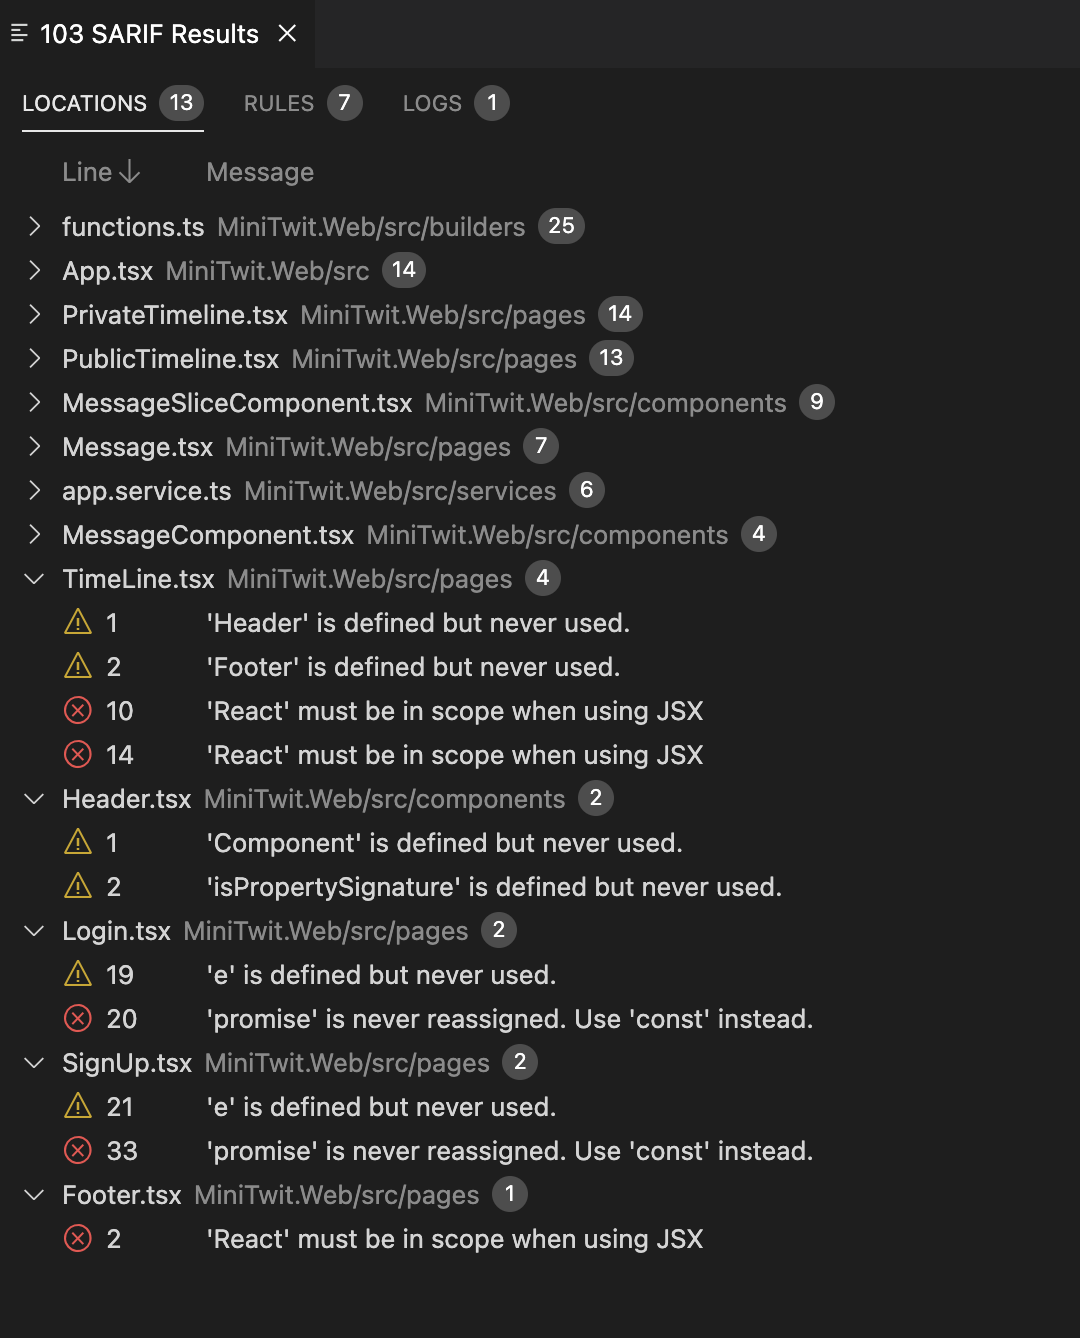
\includegraphics[width=10cm]{Eslint_report.png}
    \caption{Eslint scan - Report}
    \label{fig:elsint_report}
\end{figure}

\subsection{\texttt{snyk-security.yml}}
Pipeline that integrates with Snyk, which provide continues security monitoring. The pipeline scans the project's dependencies to identify any known vulnerabilities and automatically sets up a pull request that updates packages which are outdated or contains vulnerabilities. 

\begin{figure}[H]
    \centering
    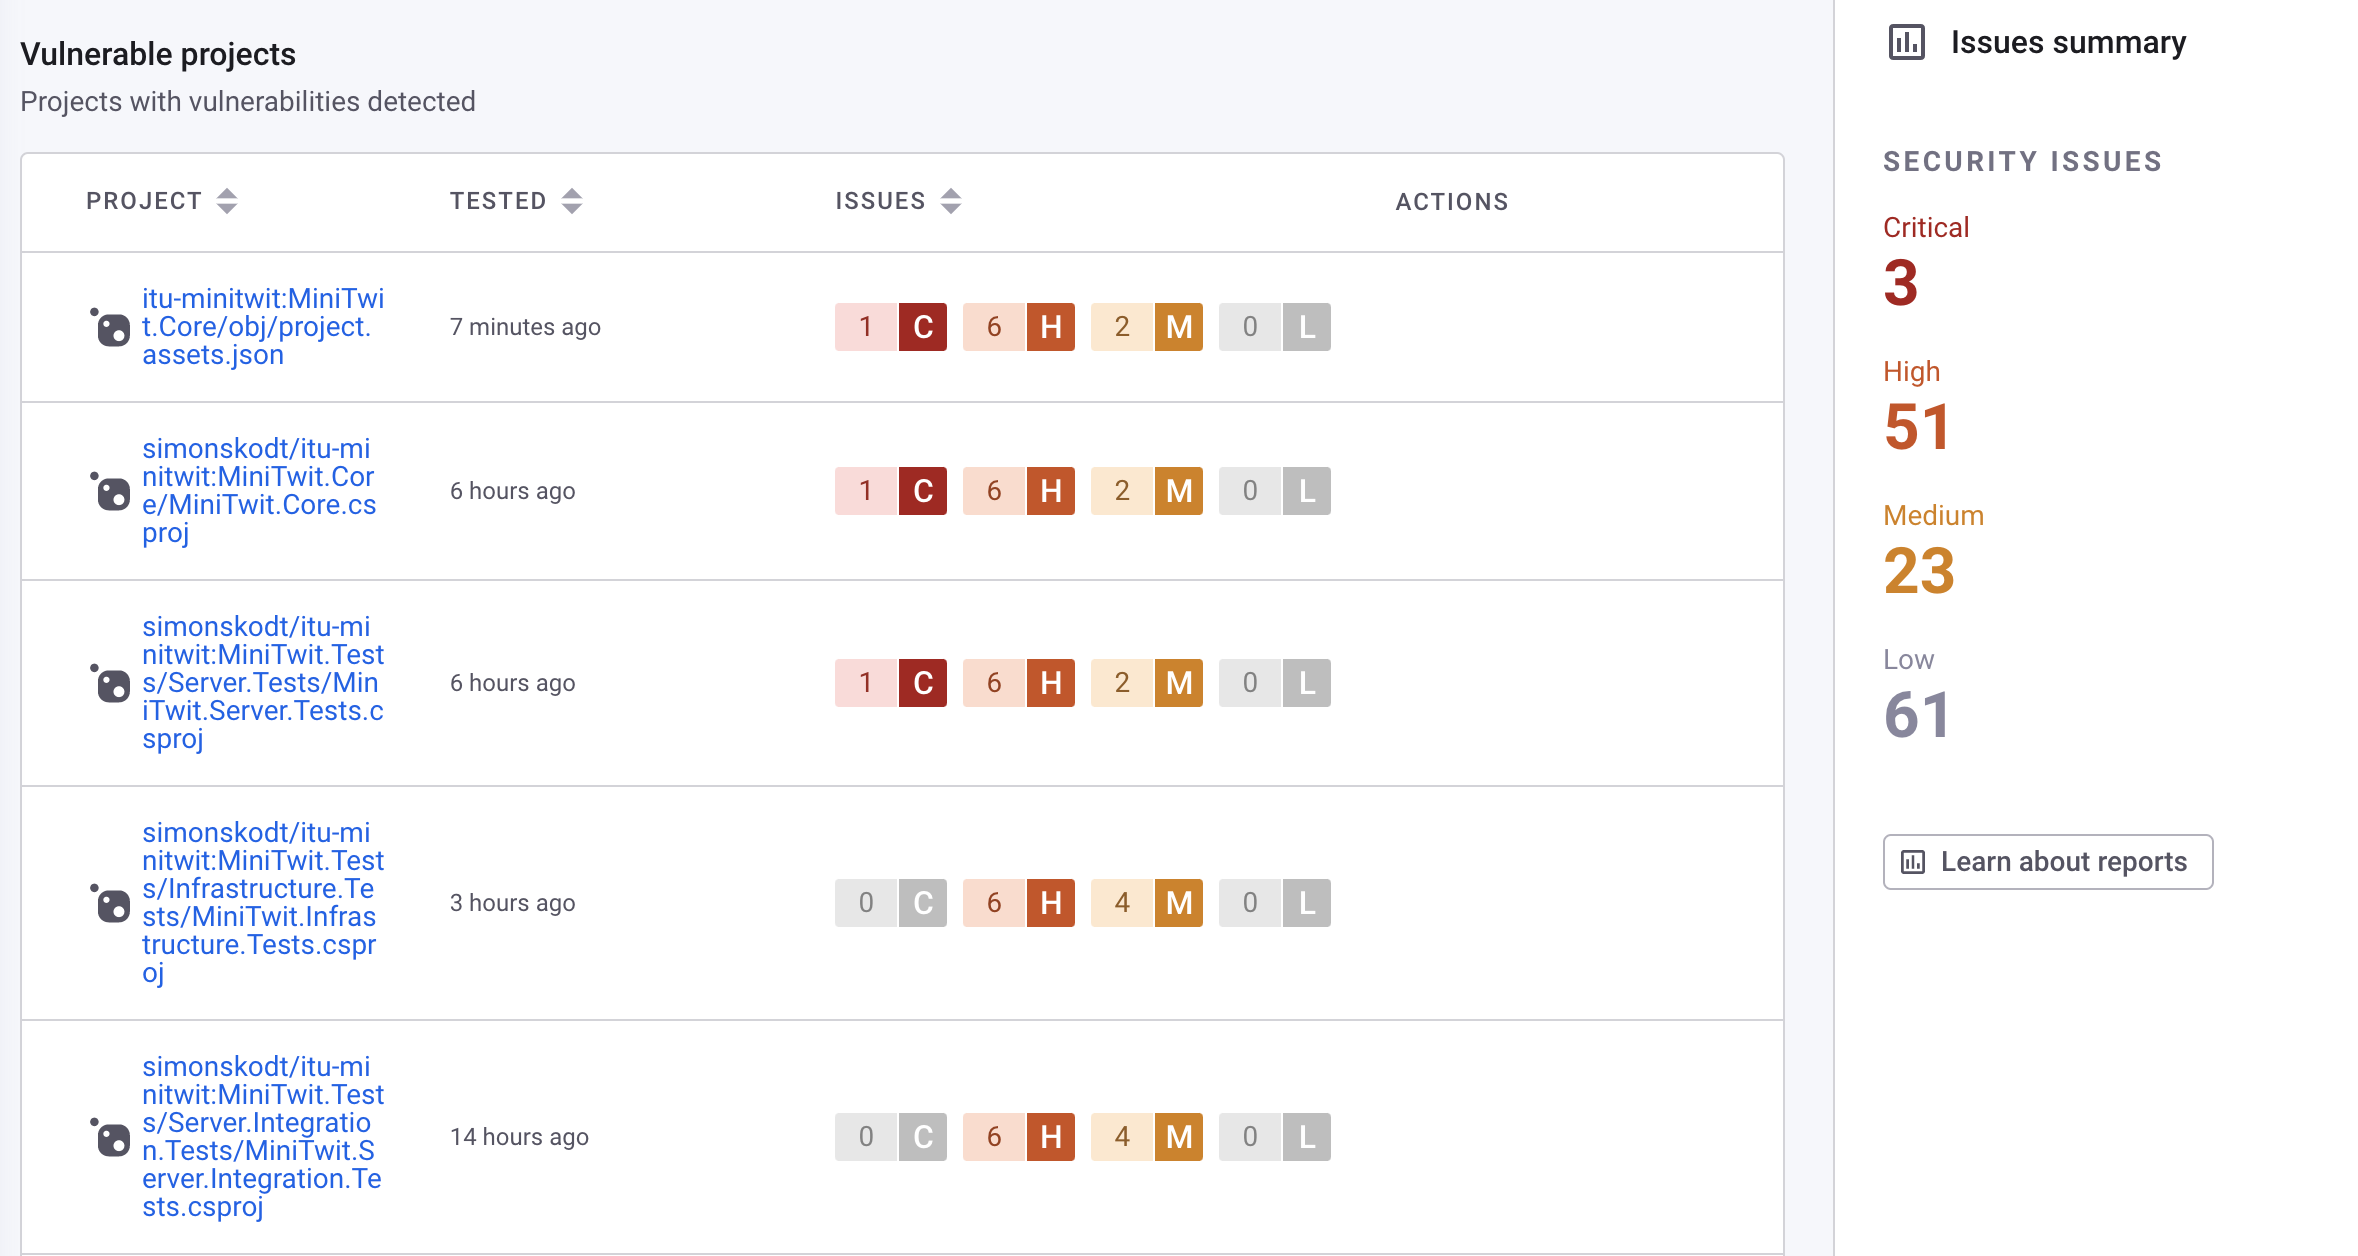
\includegraphics[width=10cm]{Snyk_report.png}
    \caption{Snyk Security - Report}
    \label{fig:snyk_report}
\end{figure}

\subsection{\texttt{continuous-deployment.yml}}
Every pipleline highlighed so far, is triggered either by pushing to a development branch or creating a PR to the main branch. The combination of these pipelines constitutes the project's \textit{deployment gate } which is a collection of predefined checks and signals that must pass before a deployment may be triggered \cite{DevOps_gates}. If the PR passes the gate, it can be deployed. This is done by mergin the PR, which will trigger the continuous-deployment pipeline.

This pipeline is separated into two jobs, namely build an deploy. The \textit{build} job is responsible for building and pushing the Docker images for the MiniTwit backend and frontend, respectively. The job uses the Docker Build tool to build the images, and then pushes them to Docker Hub.

The \textit{deploy} job is responsible for deploying the MiniTwit application and monitoring/logging components to the live server. This job is dependent on the \textit{build} job to ensure that the images are built and available for deployment. The job first uses rsync to copy the Docker Compose files and monitoring/logging configuration files to the live server. Then it uses the SSH Action to log in to the live server and deploy the MiniTwit application and monitoring/logging components by  executing the docker compose files:\textit{docker-compose.prod.yml} and \textit{docker-compose.monitoring.yml}

\section{Repository Organisation}
The group has emplyed a mono-repository approach, in which all components are stored within a single GitHub repository. While the option to maintain separate repositories for the frontend and backend existed, it was decided that, given the size of this project, a mono-repository was better with regards to the standardization of branch strategies, review of pull requests, and deployment strategy, i.e. we can deploy the whole service from a single PR.

\section{Branching Strategy}
We have used a trunk based branching strategy where where we work with two types of branches.

\begin{itemize}
    \item The main branch / trunk (long-lived)
    \item Severel feature branches (short-lived)
\end{itemize}

The main branch always contains the newest working instance of MiniTwit, the feature branches are short-lived branches containing new features for MiniTwit. As soon as a feature is completed, the feature branch is merged with the development branch by means of pull requests. Once the merge is accomplished, the feature branch is deleted. Due to branch protection rules merge request can only be accepted onto the main branch after it has undergone review, approval, and has passed all pipeline checks. In order to maintain a clean history of the version control system, it is recommended that each branch correspond to an issue on GitHub, and that commit messages has the following format.

\begin{verbatim}
    <commit type>([scope]): <message>
\end{verbatim}

\section{Monotoring}

\begin{figure}[H]
    \centering
    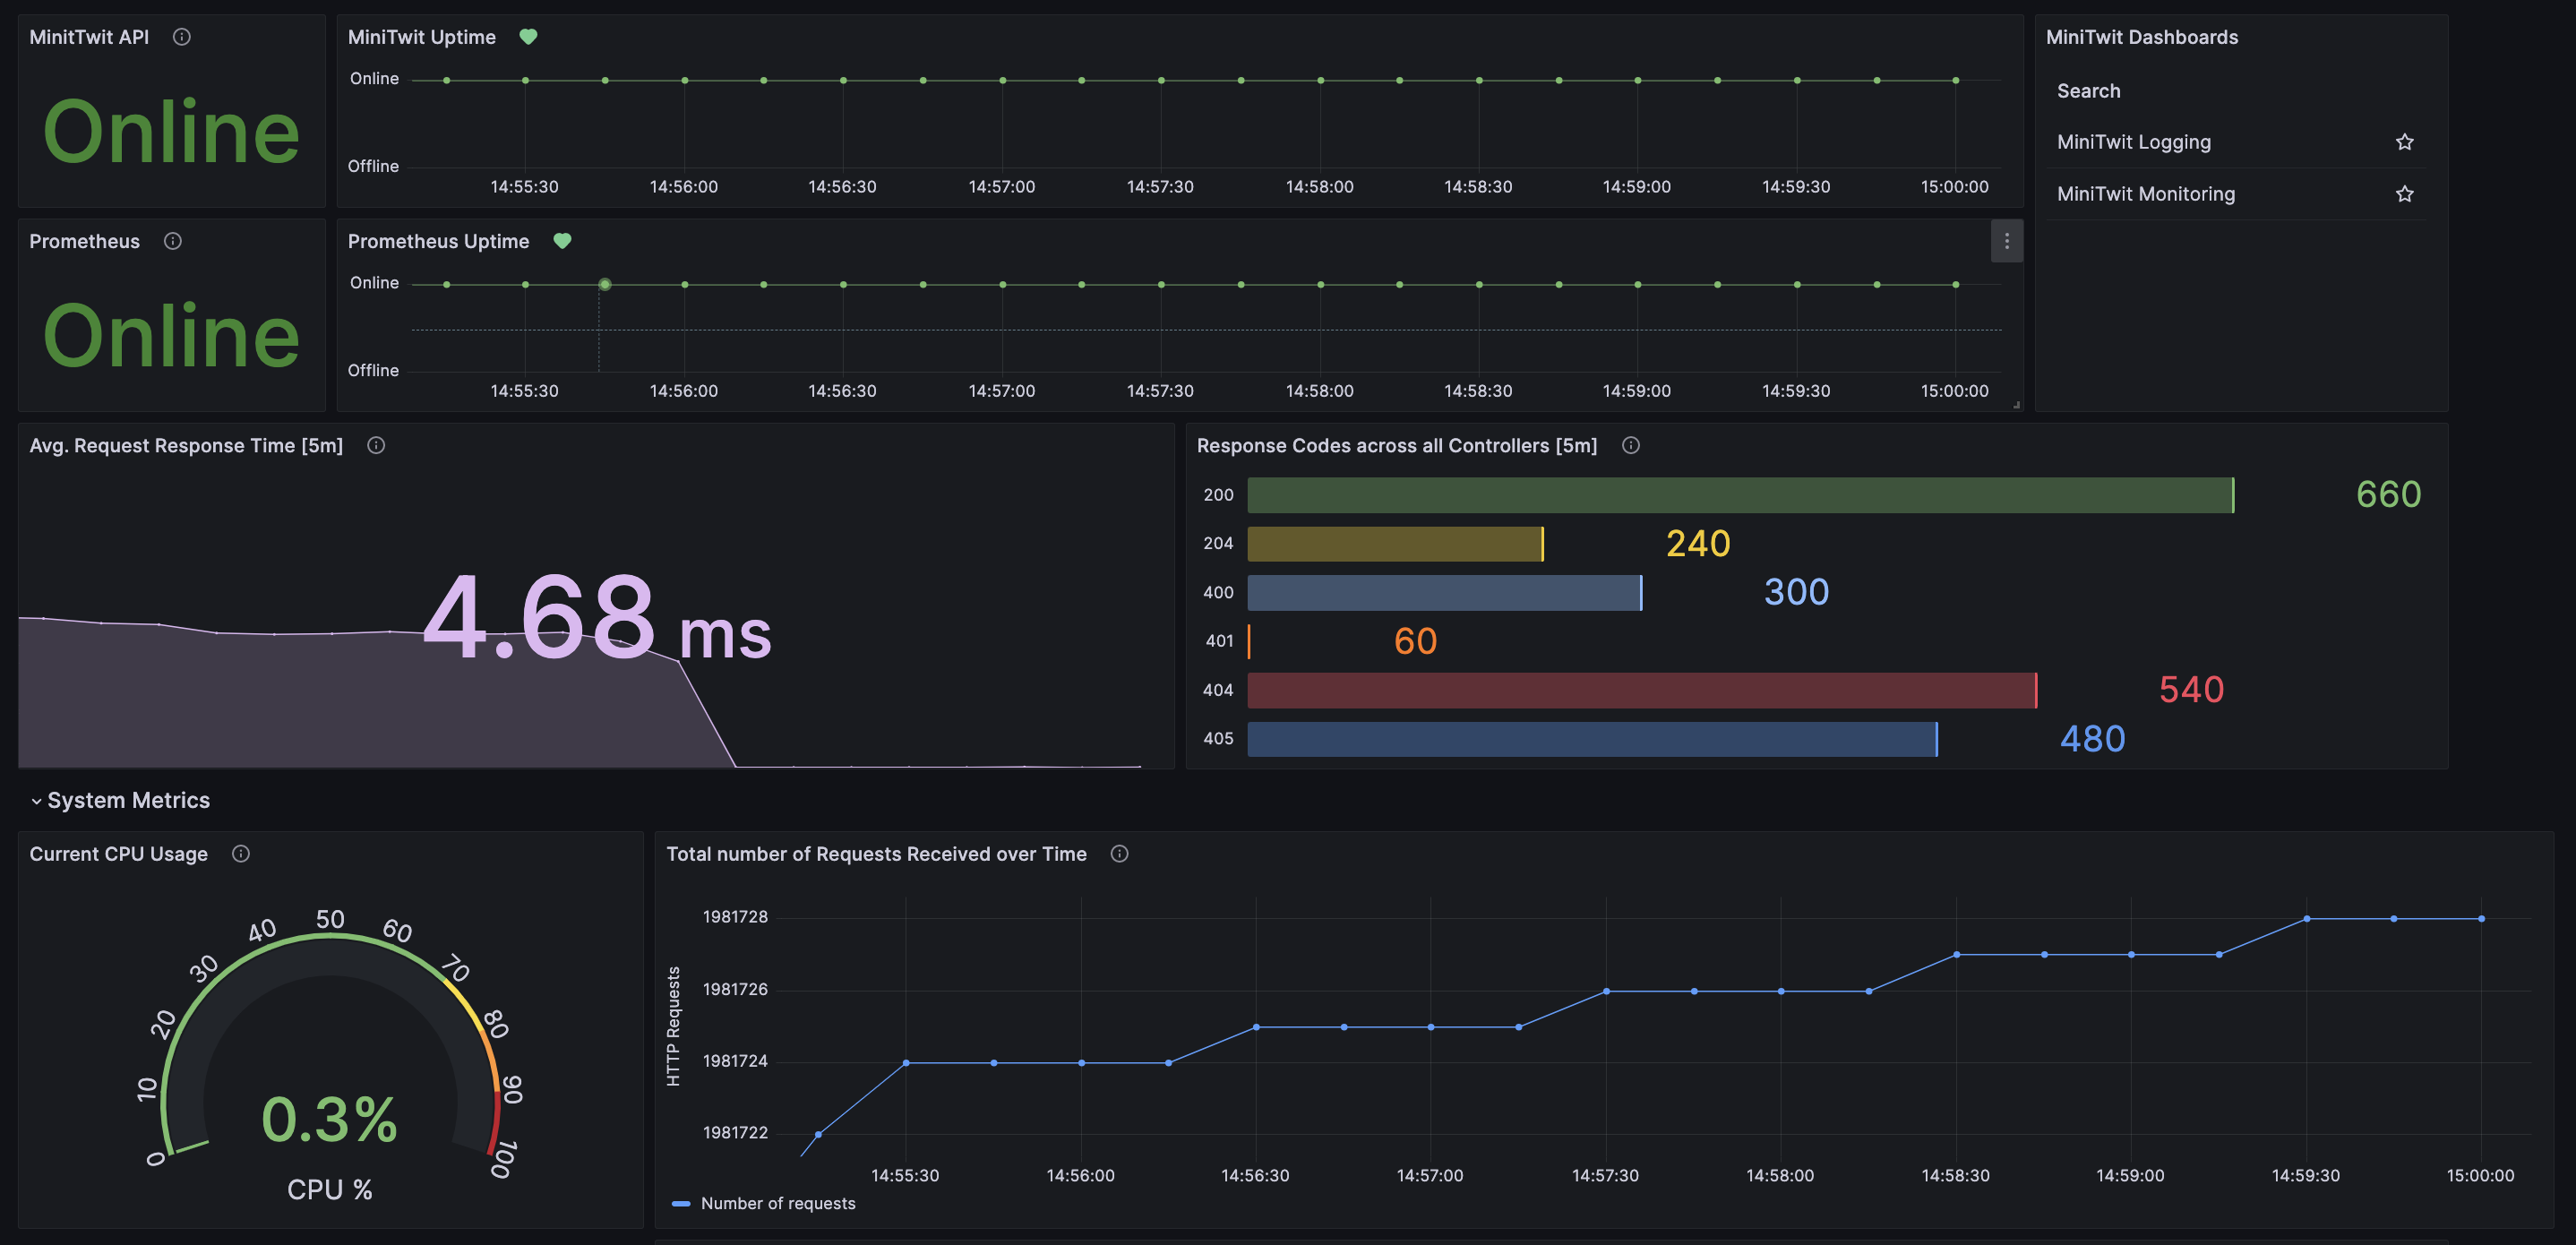
\includegraphics[width=16cm]{Monitoring.png}
    \caption{Monitoring from grafana dashboard}
    \label{fig:Minitwit_monitoring}
\end{figure}

\section{Logging}

\begin{figure}[H]
    \centering
    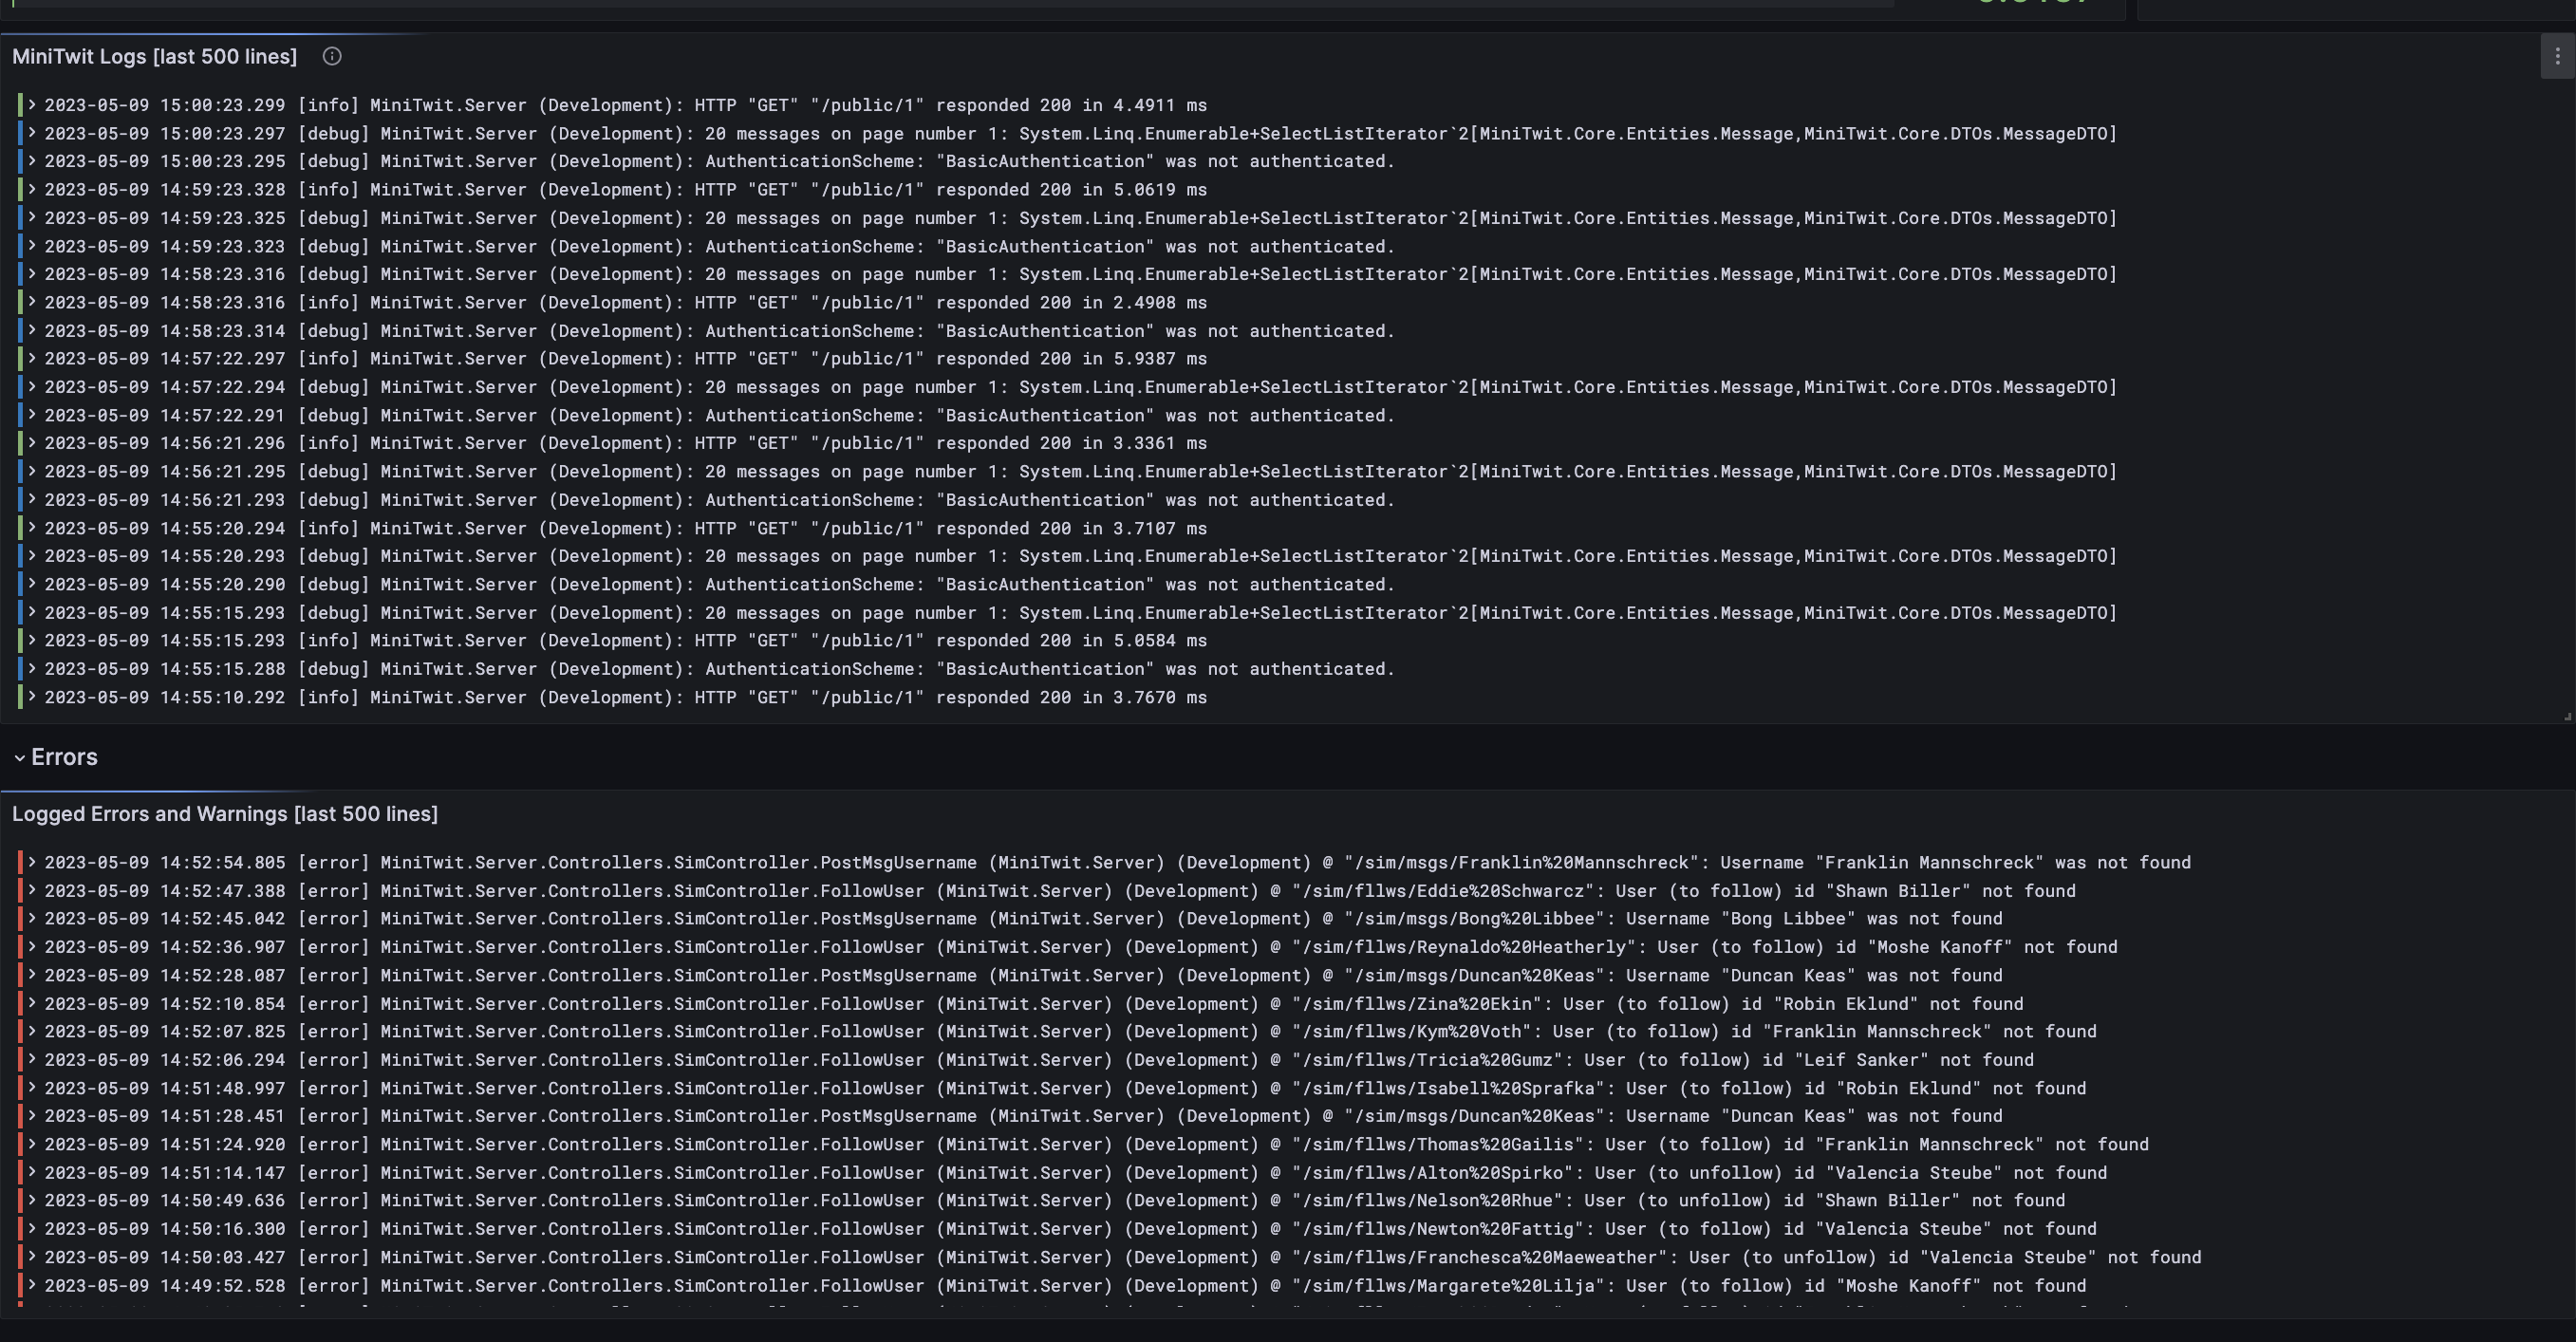
\includegraphics[width=16cm]{Logging.png}
    \caption{Logging from grafana dashboard}
    \label{fig:Minitwit_logging}
\end{figure}

\section{Security}

\section{Scaling and Load Balancing}